\documentclass[13pt,d,ukrlang]{vakthesisatu}
\synctex=1
%\documentclass[14pt]{dissatu}

%\usepackage[verbose,showframe,a4paper,tmargin=20mm,bmargin=20mm,lmargin=25mm,rmargin=20mm,headsep=4pt]{geometry}
\usepackage[verbose,a4paper,tmargin=20mm,bmargin=20mm,lmargin=25mm,rmargin=20mm,headsep=4pt]{geometry}
\newlength\TW
\setlength{\TW}{0.01\textwidth} % after geometry!

% \usepackage[backend=biber,language=russian,sorting=nty,maxnames=5,bibstyle=gost-numeric]{biblatex}
%\usepackage[backend=biber,bibstyle=gost-numeric,language=russian,sorting=nty,movenames=false,url=false,eprint=false]{biblatex}
\usepackage[backend=biber,bibstyle=gost-numeric,language=russian,sorting=nty,url=false,eprint=false]{biblatex}


\newcommand{\booknameUa}{Ансамблеві пошукові моделі і методи параметричної ідентифікації систем з хаотичною поведінкою}
\newcommand{\booknameRu}{Ансамблевые поисковые модели и методы параметрической идентификации систем с хаотическим поведением}
\newcommand{\booknameEn}{Ensemble search models and methods for parametric identification of systems with chaotic behavior}
\newcommand{\bookname}{\booknameRu}

\newcommand{\bookyear}{2018}
\newcommand{\dissauthorUa}{Гуда~А.І.}
\newcommand{\dissauthorRu}{Гуда~А.И.}
\newcommand{\dissauthorEn}{Guda~A.I.}
\newcommand{\dissauthorFullRu}{Гуда Антон Игоревич}
\newcommand{\dissauthorFullUa}{Гуда Антон Ігорович}
\newcommand{\dissauthorMain}{\dissauthorRu}
\newcommand{\dissauthorAref}{\dissauthorUa}
\newcommand{\dissauthorFullMain}{\dissauthorFullRu}
\newcommand{\dissauthorFullAref}{\dissauthorFullUa}

\newcommand{\dissSpecUa}{математичне    моделювання  та обчислювальні методи}
\newcommand{\dissSpecRu}{математическое моделирование и вычислительные методы}
\newcommand{\dissSpecEn}{Mathematical Modelling and Computational Methods}
\newcommand{\dissSpecMain}{\dissSpecRu}
\newcommand{\dissSpecAref}{\dissSpecUa}
\newcommand{\dissSpecId}{01.05.02}
\newcommand{\dissScopeRu}{технических наук}
\newcommand{\dissScopeUa}{техничних наук}
\newcommand{\dissScopeMain}{\dissScopeRu}
\newcommand{\dissScopeAref}{\dissScopeUa}
\newcommand{\UDC}{004: 681.5.015}
\newcommand{\dissRada}{Д.~08.084.01}
\newcommand{\dissSekrRadi}{Селівьорстова~Т.В.}
\newcommand{\institutionRu}{Национальная металлургическая академия Украины}
\newcommand{\institutionUa}{Національна  металургійна     академія України}
\newcommand{\institutionEn}{National Metallurgical academy of Ukraine}
\newcommand{\institutionMain}{\institutionRu}
\newcommand{\institutionAref}{\institutionUa}
\newcommand{\belongRu}{Министерство образования и науки Украины}
\newcommand{\belongUa}{Міністерство освіти і науки      України}
\newcommand{\belongEn}{Ministry of Education and Science of Ukraine}
\newcommand{\belongMain}{\belongRu}
\newcommand{\belongAref}{\belongUa}
\newcommand{\cityRu}{Днепр}
\newcommand{\cityUa}{Дніпро}
\newcommand{\cityEn}{Dnipro}
\newcommand{\cityMain}{\cityRu}
\newcommand{\cityAref}{\cityUa}
\newcommand{\superRu}{Михалёв Александр Ильич}
\newcommand{\superUa}{Михальов Олександр Ілліч}
\newcommand{\superMain}{\superRu}
\newcommand{\superAref}{\superUa}



\hypersetup{
  breaklinks=true,
  linktocpage=true,
  bookmarksnumbered,
  colorlinks=true,
  linkcolor=black,
  urlcolor=black,
  citecolor=black,
  pdfkeywords={chaotic systems,identification criterion,searching agent,searching coordinator,ensemble methods of the searching indetification.}
}
%  pdftitle={\thetitle},
%  pdfauthor={\theauthor},
% pdftitle
%  linkcolor=blue,
  %urlcolor=urlcolor,
% pdfauthor
% pdfsubject
% pdfcreator
% pdfproducer
% pdfkeywords
% pdftrapped
\urlstyle{rm}

\usepackage{blox}
\usepackage[europeanresistors,americaninductors,siunitx,fulldiodes]{circuitikz}

\usetikzlibrary{calc}
\usetikzlibrary{arrows}
\usetikzlibrary{patterns}
%\usepgflibrary{shapes.geometric}
\usetikzlibrary{external}


\definecolor{haircolor}{rgb}{0.7,0.7,1.0}
\newcommand{\TikzAddPadding}{\path (current bounding box.north east) ++(+0.1,+0.1); \path (current bounding box.south west) ++(-0.1,-0.1);}

\tikzset{
  >=stealth,
  %semiRed/.style={fill=red,opacity=0.3,draw=black,thin},
  hair/.style={draw,color=haircolor,line width=0.1pt},
  medline/.style={draw=black,line width=0.6pt},
  medlinep/.style={draw=black,line width=0.6pt,->},
  semiboldline/.style={draw=black,line width=1.2pt},
  semiboldlinep/.style={draw=black,line width=1.2pt,->},
  infoline/.style={draw=gray,line width=1.4pt},
  boldline/.style={draw=black,line width=2.0pt},
  boldlinep/.style={draw=black,line width=2.0pt,->},
  wire/.style={draw=black,line width=1.0pt},
  elelem/.style={draw=black,line width=1.5pt},
  subelem/.style={draw=black,dashed,line width=0.6pt}
}




\renewcommand{\Rada}{\dissRada}
\renewcommand{\SekrRadi}{\dissSekrRadi}

\author{\dissauthorFullRu}

\title{\bookname}
\supervisor{\superMain}{д.т.н., проф.}
\date{\bookyear}

%\setstretch{1.2}



\addbibresource{atuworks.bib}
\addbibresource{artrefs.bib}

\hypersetup{
  pdftitle={\bookname},
  pdfauthor={\dissauthorMain},
  colorlinks=true,
  linkcolor=blue,
  citecolor=brown
}

%\newcommand{\LinkRef}[1]{ \textit{\color{red}#1} }
\newcommand{\LinkRef}[1]{}
\newcommand{\Cmt}[1]{ {\small\color{red}#1\color{black}.} }
%\newcommand{\Cmt}[1]{}

\clubpenalty9990
\widowpenalty9990%

%\pagestyle{stheadings}

% ====================================================================================================
\begin{document}

\thispagestyle{empty}
\Xmaketitle
% \begin{center}
%   {\Large Титульная страница}
%   \vfill
%   \bookyear
% \end{center}


\clearpage

\phantomsection
\pdfbookmark[0]{АНОТАЦІЯ}{annotauabookmark}

\begin{center}
\textbf{АНОТАЦІЯ}
\end{center}

\medskip

\textit{\dissauthorUa} \booknameUa.
--- Кваліфікаційна робота на правах рукопису.

Дисертація на здобутті наукового ступеня доктора технічних наук за спеціальністю
\dissSpecId ``\dissSpecUa''. --- \institutionUa, \belongUa, \bookyear.


Робота присвячена актуальній науково-технічній проблемі
ідентифікації параметрів складних технічних систем у режимі хаотичної динаміки.
Нелінійні динамічні системи, розповсюджені в сучасних технологічних і
природних процесах, можуть проявляти хаотичні властивості в своїй динаміці.
Існуючи системи ідентифікації нелінійних динамічних об'єктів практично не
здатні функціонувати у таких умовах.
Проаналізовано існуючи методи ідентифікації та моделі динаміки пошуку.
Визначено спільні риси систем ідентифікації,
досліджено чинники, які не дозволяють використовувати їх
для ідентифікації параметрів хаотичних систем.
Обґрунтована необхідність створення нових систем ідентифікації.

Об'єктом дослідження є 
технічні системи, які в процесі їх функціювання можуть
входити в хаотичні режими.

Предметом дослідження є
математичні моделі процесів та методи
ансамблевої ідентифікації технічних систем з хаотичною динамікою.

Методи дослідження:
Для вирішення поставлених задач використовувався математичний апарат
теорії управління та ідентифікації нелінійних систем, динамічного хаосу,
обчислювальних методів, нечіткої логіки, теорії інформації тощо.

Практичне значення отриманих результатів полягає у тому,
що озроблені методи ідентифікації було використано
при проектуванні, створенні, налаштовуванні параметрів
стенду дослідження вібраційного та акустичного впливу.
Аналіз результатів даних з цього стенду
дав можливість вказати необхідні нелінійні властивості системи
та діапазон параметрів, які у сукупності
забезпечують широкосмуговий спектр коливань.

Створене програмне середовище для моделювання нелінійних динамічних систем
використовується при проведенні практичних робіт по дисциплінам
``Моделювання систем'',
``Сучасні системи управління'' на кафедрі інформаційних технологій
і систем Національної металургійної академії України.

В дисертаційній роботі
  створено критерії ідентифікації нелінійних динамічних систем,
  які, на відміну від тих, що існують, дозволяють оцінити їх стан та
  хаотичну динаміку, а також дають підстави для створення ефективних алгоритмів
  настроювання параметрів моделей систем ідентифікації.

Створено методи ідентифікації на підставі
  адаптивно-пошукової парадигми з використанням ансамблю пошукових агентів,
  які взаємодіють проміж собою, які на відміну від методів, що використовують
  одну модель або пару моделей, значно підвищують швидкість пошуку та
  здатні за мінімальний час  перелаштовуватися при різкій зміні параметрів, а на
  відміну від ройових алгоритмів нові методи потребують значно меншої
  кількості моделей та забезпечують певні гарантії пошуку.

Створено нову класифікацію систем ідентифікації динамічних систем,
  яка, як вбирає у себе методи, що існують, так і дозволяє
  створювати нові методи ідентифікації за рахунок
  комбінування їх складових частин;

Запропоновано модель системи хаотичної динаміки
   з використанням зв'язаних релаксаційних генераторів,
   яка відрізняється від існуючих відсутністю індуктивних компонентів,
   працездатністю при малих напругах та можливістю
   керування частотним діапазоном у широкому інтервалі,
   що сприяє процесу аналізу хаотичної динаміки
   фізичного об'єкту, перевірці адекватності математичної моделі
   та властивостей системи ідентифікації.

Вдосконалено
  методи оцінювання якості ідентифікації,
  які на відміну від тих, що існують,
  враховують використання множини агентів.

Набуло подальший розвиток
  підходи до адаптації параметрів систем
  ансамблевої ідентифікації, які придатні використовувати поточну
  інформацію від ансамблю синергірованих моделей та коригувати глобальні
  параметри пошуку в умовах апріорної та поточної невизначеності.

Вдосконалено
модель генератора Колпітца, яка враховує
    більшу кількість нелінійних ефектів,
    що забезпечує більш адекватні результати процесу
    ідентифікації її параметрів запропонованими методами.

Встновлено, що
для вирішення завдання ідентифікації необхідно існування
критерію, що відображає схожість динаміки об'єкта і моделей.
    У тих випадках, коли утруднено формування критерію на
    підставі чітких фізичних принципів, має сенс вид критерію
    отримати перебором, заснованому на обмеженій множині уявлень
    інтегральних величин.

    Саме поняття інтегрального критерію має на увазі певний
    вид усереднення, що в певній мірі відповідає застосуванню
    низькочастотної фільтрації.

    Застосування функцій якості ідентифікації необхідно для
    визначення досягнення мети ідентифікації, отримання значення
    ідентифікованого параметра координатором пошуку. Деякі методи
    роботи пошукових агентів вимагають значень цих функцій в якості
    вхідного сигналу.

    Встановлено основні вимоги до властивостей функцій якості
    ідентифікації, розглянуті основні способи визначення.

    Визначено набір структур систем ідентифікації, заснованих на
    взаємодії пошукових агентів і координаторів пошуку. Визначено
    підклас системи ідентифікації, що використовують при своїй
    роботі динаміку ансамблю пошукових агентів.

    Визначено методи локальної оцінки значення ідентифікованого
    параметра як для пошукових агентів, які використовують значення
    як критерію, так і функції якості.

    Визначено способи завдання динаміки пошукових агентів.
    Визначено методи отримання значення ідентифікованого параметра
    координатором пошуку.

    Створена класифікація ансамблевих пошукових систем, що дозволяє
    коротким і однозначним чином визначити структуру і динаміку,
    а також створювати нові методи, за умови визначення правил
    роботи елементів пошукових агентів і координаторів пошуку.

    На простих не динамічних тестових завданнях вивчені базові
    властивості як окремих елементів ансамблевих систем
    ідентифікації, так і систем в цілому.

Результати було впроваджено у рамках науково-практичного дослідження
``Оцінка можливості заміни випробувань КА на стійкість до акустичного навантаження
випробуваннями широкосмугової вібрації'', згідно договору \hbox{№~V-105-16-3} від 07.09.2016
(Спеціальне конструкторсько-технологічне бюро ІТМ НАН України, м.~Дніпро),
та при ідентифікації режиму роботи вертикально-осьової вітроустановки з H-ротором Дар'є
з врахуванням складно-періодичної або хаотичної структури коливань лопатей
(Інститут транспортних систем і технологій НАН України, м.~Дніпро).

\textbf{Ключові слова:}
хаотичні системи,
критерій ідентифікації,
пошуковий агент,
координатор пошуку,
ансамблеві методи пошукової ідентифікації.









\clearpage

\phantomsection
\pdfbookmark[0]{АBSTRACT}{annotarnbookmark}

\begin{center}
\textbf{АBSTRACT}
\end{center}

\medskip

\textit{\dissauthorEn} \booknameEn.
---
Qualifying scientific work as a manuscript.

Thesis for obtaining the doctoral degree in technical sciences in the specialty
\dissSpecId ``\dissSpecEn''. --- \institutionEn, \belongEn, \bookyear.

The dissertation is devoted to the actual scientific and technical problem of
identifying the complex technical systems parameters in the chaotic dynamics regime.
Nonlinear dynamic systems are usual in modern technological and natural processes,
and can exhibit chaotic properties in their dynamics.
The existing systems for identifying nonlinear dynamic objects are practically
useless in such conditions.

The existing identification methods and search dynamics models are analyzed.
Identified common features of identification systems, investigated factors that
do not allow them to be used in the parameter identification task for chaotic systems.
The necessity of creating new identification systems is grounded.

It is shown that the use of integral criteria is necessary
for the identification systems creation, that would be workable under conditions of chaotic
dynamics. Considered a couple of physical justification for the criteria syntesys,
both on the direct use of physical laws, and on empirical principles.

In order to improve the identification system speed,
a structure. which consist of a variety search agents and a search coordinatoris is proposed.
Methods for estimating the parameter of the triplet of search agents are created, both with
the direct use of the criterion and with the use of the quality function. The
dependence of the identification error on the method and its parameters is
investigated.

A group of methods for the work of the search coordinators has been created,
the dependencies of the identification quality on the parameters of the
coordinator's interaction with the agents have been determined. A
classification of system identification systems has been created, which allows
not only briefly describe the set of methods used, but also allows us to
create new identification systems when new methods of agents and coordinators
appear. The properties of the set of proposed methods for an artificial
quasistationary test system are investigated. A subset of methods is selected,
which it is expedient to use in further research.

The ``qontrol'' software was created, which is intended for modeling complex
nonlinear dynamical systems, including in the analysis of chaotic dynamics systems processes identification.

The working capacity and properties of the developed methods have been verified
in solving the problem of identifying several nonlinear systems, both known
chaotic dynamics systems, and new ones. It was determined that there are
systems that are not chaotic, but from the point of view of identification they
have common features. The influence of the parameters of the identification
system on the quality of its work is investigated, which gives grounds for the
adaptation of these parameters. It is determined that the type of criterion and
the dynamics of agents have the greatest influence.

The properties of the proposed identification methods are investigated on two
real physical objects: the Kolpitts oscillator and the system of coupled
relaxation elements. The methods have confirmed their efficiency, and it is
found that the dependence of the quality of identification on its parameters
for real systems has the same form as for the test ones.


\textbf{Keywords:}
chaotic systems,
identification criterion,
searching agent,
searching coordinator,
ensemble methods of the searching indetification.


\medskip

\begin{center}
Список публікацій здобувача
\end{center}

\begin{enumerate}



\item
Гуда А. И., Михалёв А. И., Новикова Е. Ю. Синтез критерия идентификации нелинейных
динамических систем на физических принципах // Адаптивнi системи автоматичного
управлiння. Мiжвiдом. науково-техн. зб. (РИНЦ). --- Днепропетровск, 2008. --- 11(31). --- С. 136--142.

\item
Гуда А. И., Михалёв А. И. Адаптивно-поисковая идентификация хаотической динамической
системы Дуффинга // Адаптивнi системи автоматичного управлiння.
Мiжвiдом. науково-техн. зб. (РИНЦ). --- Днепропетровск, 2008. --- 12(32). --- С. 166--171.

\item
Гуда А. И., Михалёв А. И. Адаптивно-поисковая идентификация хаотической динамической
системы Рёсслера // Адаптивнi системи автоматичного управлiння. Мiжвiдом.
науково-техн. зб. (РИНЦ). --- Днепропетровск, 2009. --- 14(34). --- С. 125--129.

\item
Guda A. I., Mikhalyov A. I. Multi-model methods and parameters estimation approaches
on non-linear dynamic system identification // Системнi технологiї. Регiональний мiжвузiвський
збiрник наукових праць (Index Copernicus). --- Днепропетровск, 2015. --- 4(99). --- С. 3--9.

\item
Guda A. I., Mikhalyov A. I. Multi-model identification system properties near extremum:
simulations and analysis // Journal of Applied Computer Science – JACS-2015. --- 2015. --- 23(2). --- С. 21--28.

\item
Гуда А. И., Михалёв А. И. Выбор критерия при адаптивно-поисковой идентификации
динамической системы Ван-Дер-Поля // Адаптивнi системи автоматичного управлiння.
Мiжвiдом. науково-техн. зб. (РИНЦ). --- Днепропетровск, 2010. --- 16(36). --- С. 154--160.

\item
Гуда А. И., Михалёв А. И. Использование нечётких технологий при выборе начальных
условий в задачах идентификации систем с хаотической динамикой // Адаптивнi системи
автоматичного управлiння. Мiжвiдом. науково-техн. зб. (РИНЦ). --- Днепропетровск, 2014. --- 2(25). --- С. 98--103.

\item
Guda A. I., Mikhalyov A. I. Method of Lorenz systems parametric identification by the
searching models ensemble // Scientific and Technical Conference ``Computer Sciences and
Information Technologies'' (CSIT) (Scopus). --- 2015. --- С. 73--75. --- DOI: 10.1109/STC-CSIT.2015.7325435.

\item
Гуда А. И., Михалёв А. И. Информационные оценки сложности задачи параметрической
идентификации динамических систем // Адаптивнi системи автоматичного
управлiння. Мiжвiдом. науково-техн. зб. (РИНЦ). --- Днепропетровск, 2007. --- 10(30). --- С. 96--103.

\item
Гуда А. И., Михалёв А. И., Деревянко А. И. Критерии идентификации параметров хаотической
динамики управляемого объекта // Автомобiльний транспорт. – Вiсник Харкiвського
нацiонального автодорожнього унiверситету. --- 2009. --- No 25. --- С. 254--257.

\item
Гуда А. И., Михалёв А. И. Влияние возмущений входного сигнала на динамику и
идентификацию нелинейной системы Дуффинга // Адаптивнi системи автоматичного
управлiння. Мiжвiдом. науково-техн. зб. (РИНЦ). --- Днепропетровск, 2010. ---
15(35). --- С. 121--125.

\item
Гуда А. И., Михалёв А. И. Исследование альтернативного критерия при адаптивно-поисковой
идентификации динамической системы Ван-Дер-Поля // Адаптивнi системи автоматичного управлiння.
Мiжвiдом. науково-техн. зб. (РИНЦ). --- Днепропетровск, 2010. --- 17(37). --- С. 149--154.

\item
Гуда А. И., Михалёв А. И. Сравнительный анализ двух критериев адаптивно-поисковой
идентификации нелинейной динамической системи Ван-Дер-Поля // Системнi технологiї.
Регiональний мiжвузiвський збiрник наукових праць. --- Днепропетровск,
2011. --- 4(75). --- С. 15--20.

\item
Гуда А. И., Михалёв А. И. Синтез критерия при адаптивно-поисковой идентификации
динамической системы Чуа // Адаптивнi системи автоматичного управлiння. Мiжвiдом.
науково-техн. зб. (РИНЦ). --- Днепропетровск, 2011. --- 18(38). --- С. 140--146.

\item
Гуда А. И., Михалёв А. И., Дмитриева И. С. Особенности моделирования и идентификации
хаотической системы Ресслера с возмущениями // Системнi технологiї. Регiональний
мiжвузiвський збiрник наукових праць. --- Днепропетровск, 2010. --- 2(67). --- С. 114--118.

\item
Гуда А. И., Михалёв А. И. Моделирование и исследование хаотической динамики связанных
релаксационных генераторов // Адаптивнi системи автоматичного управлiння.
Мiжвiдом. науково-техн. зб. (РИНЦ). --- Днепропетровск, 2011. --- 19(39). --- С. 164--170.

\item
Гуда А. И., Михалёв А. И. Физические основы при синтезе критерия адаптивно-поисковой
идентификации динамической системы Лоренса // Системнi технологiї. Регiональний мiжвузiвський
збiрник наукових праць. --- Днепропетровск, 2012. --- 2(79). --- С. 13--19.

\item
Guda A. I., Mikhalyov A. I. Chaotic system with relay hysteresis in return force: simulation
and analysis // Системнi технологiї. Регiональний мiжвузiвський збiрник наукових
праць (Index Copernicus). --- Днепропетровск, 2013. --- 2(85). --- С. 30--35.

\item
Гуда А. И., Михалёв А. И. Моделирование хаотической динамики системы с зоной
нечувствительности и идентификация её параметров // Адаптивнi системи автоматичного
управлiння. Мiжвiдом. науково-техн. зб. (РИНЦ). --- Днепропетровск, 2012. ---
20(40). --- С. 180--186.

\item
Гуда А. И., Михалёв А. И. Генератор Колпитца: моделирование хаотической динамики
и параметрическая идентификация // Адаптивнi системи автоматичного управлiння.
Мiжвiдом. науково-техн. зб. (РИНЦ). --- Днепропетровск, 2012. --- 21(41). --- С. 146--153.

\item
Guda A. I., Mikhalyov A. I. Influence of input and measurement noise to Lorenz system
adaptive-searching identification // Системнi технологiї. Регiональний мiжвузiвський
збiрник наукових праць (Index Copernicus). --- Днепропетровск, 2014. --- 2(91). --- С. 154--158.

\item
Гуда А. И., Михалёв А. И. Настройка адаптивно-поисковой системы идентификации применительно
к хаотическим объектам // Адаптивнi системи автоматичного
управлiння. Мiжвiдом. науково-техн. зб. (РИНЦ). --- Днепропетровск, 2013. --- 1(22). ---
С. 134--139.

\item
Гуда А. И., Михалёв А. И. Расширение рабочего диапазона поисковой идентификации
нелинейных динамических систем // Адаптивнi системи автоматичного управлiння.
Мiжвiдом. науково-техн. зб. (РИНЦ). --- Днепропетровск, 2013. --- 2(23). --- С. 133--127.

\item
Гуда А. И., Михалёв А. И. Повышение качества фильтрации при поисковой идентификации
нелинейных динамических систем // Адаптивнi системи автоматичного
управлiння. Мiжвiдом. науково-техн. зб. (РИНЦ). --- Днепропетровск, 2014. --- 1(24). --- С. 160--165.

\item
Physical background in identification criterion synthesis / A. I. Guda, A. I. Mikhalyov,
A. I. Derevjanko, P. Kisa la // Elektronika konstrukcje, technologie, zastosowania (Index
Copernicus). --- 2013. --- No 8. --- С. 32--34.

\item
Гуда А. И., Михалёв А. И. Расширение рабочего диапазона при поисковой идентификации
хаотической системы Чуа // Вестник Херсонского национального технического
университета"(РИНЦ). --- 2014. --- 3(50). --- С. 265--258.

\item
Гуда А. И., Михалёв А. И. Использование метода идентификации с множеством
подвижных моделей применительно к динамической системе Лоренса // Адаптивнi системи
автоматичного управлiння. Мiжвiдом. науково-техн. зб. (РИНЦ). --- Днепропетровск, 2015.
--- 1(26). --- С. 191--197.

\item
Система поддержки принятия решений по повышению эффективности гидроаеродинамических
процессов во вспомогательных элементах энергетических агрегатов /
Е. А. Арсирий, С. Г. Антощук, В. А. Арсирий, А. И. Гуда // Управляющие системы и машины (РИНЦ).
--- 2015. --- No 6. --- С. 43--50.

\item
Гуда А. И., Михалёв А. И. Настройка параметров системы мультимодельной
адаптивно-поисковой системы идентификации // Вестник Херсонского национального
технического университета"(РИНЦ). --- 2015. --- 3(54). --- С. 138--243.

\item
Guda A. I., Mikhalyov A. I. Multi-model methods and parameters estimation approaches
on non-linear dynamic system identification // Системнi технологiї. Регiональний мiжвузiвський
збiрник наукових праць (Index Copernicus). --- Днепропетровск, 2016. --- 2(103). --- С. 57--62.

\item
Визначення гранулометричного складу матерiалу у повiтряному потоцi з використанням
дiаграм Пуанкаре / Р. О. Сухомлин, А. И. Михальов, Н. С. Прядко, К. В. Тернова, А. И. Гуда
// Системнi технологiї. Регiональний мiжвузiвський збiрник наукових
праць (Index Copernicus). --- Днепропетровск, 2016. --- 4(105). --- С. 18--24.

\item
Гуда А. И. A low-voltage coupled relaxation generator with chaotic behavior: simulation,
measurement and identification // Системнi технологiї. Регiональний мiжвузiвський
збiрник наукових праць (Index Copernicus). --- Днепропетровск, 2016. --- 4(105). --- С. 57--65.

\item
Guda A. I., Mikhalyov A. I. Three-model methods for extremum extimation in non-linear
dynamic system identification // Адаптивнi системи автоматичного управлiння.
Мiжвiдом. науково-техн. зб. (РИНЦ). --- Днепропетровск, 2016. --- 2(27). --- С. 160--165.

\item
Зимогляд А. Ю., Гуда А. И. Особливостi використання HX711 для отримання даних з
тензодатчика // Системнi технологiї. Регiональний мiжвузiвський збiрник наукових
праць (Index Copernicus). --- Днепропетровск, 2016. --- 3(104). --- С. 136--140.

\item
Левченко Д., Гуда А. И. Виявлення залежностi кута повороту сервоприводу вiд вхiдного
iмпульсу // Системнi технологiї. Регiональний мiжвузiвський збiрник наукових праць
(Index Copernicus). --- Днепропетровск, 2016. --- 3(104). --- С. 141--146.

\item
Гуда А. И., Михалёв А. И. Синтез критерия для идентификации хаотической системы ``Sprott A''
с использованием мультимодельного адаптивно-поискового метода //
Вестник Херсонского национального технического университета"(РИНЦ). --- Херсон,
2016. --- 3(58). --- С. 204--207.

\item
Guda A. I., Mikhalyov A. I. Multi-models identification methods comparison in the non-linear
dynamic system identification task // Радиоэлектроника, информатика, управление (Web of Science).
--- Запорiжжя, ЗНТУ, 2016. --- No 4. --- С. 112--119. --- DOI: 10 . 15588/1607-3274-2016-4-14.

\item
Гуда А. И., Михалёв А. И. Оценивание эффективности применения интегральных критериев в задачах
параметрической идентификации хаотических систем // Коллективная монография
``Системные технологии моделирования сложных систем'' под. ред.
Михалёва А.И. --- Днепр, 2016. --- С. 200--229.

\item
Гуда А. И., Михалёв А. И. Выбор критериев для оценки эффективности процессов идентификации
систем с хаотической динамикой // Матерiали Всеукраїнської науково-практичної конференцiї
``Iнформатика та системнi науки'' (IСН-2011).
--- Полтава, 17-19.03.2011. --- Полтава: РВВ ПУЕТ. --- 2011. --- С. 355.

\item
Гуда А. И., Михалёв А. И. Идентификация систем с хаотической динамикой
// Материалы международной конференции ``Интеллектуальные системы принятия решений и
проблемы вычислительного интеллекта'' (ISDMCI) (май 2011).
--- Херсон: ХНТУ : ХН-ТУ, 2011. --- С. 211--212.

\item
Гуда А. И., Михалёв А. И. Адаптивно-поисковая идентификация нелинейной динамической
системы Ван-дер-Поля // Информационные технологии в управлении сложными системами.
Сборник докладов научной конференции – Днепропетровск:
изд-во ``Свидлер А.Л.'' --- Днепропетровск, 07.2011. --- С. 39--40.

\item
Гуда А. И., Михалёв А. И. Адаптивно-поисковая идентификация нелинейной хаотической
системы Чуа // Материалы международной научно-технической конференции
``Автоматизация: проблемы, идеи, решения'' (сент. 2011). --- Севастополь : СевНТУ,
2011. --- С. 18--19.

\item
Гуда А. И., Михалёв А. И. Альтернативный критерий идентификации хаотической системы Рёсслера
// Материалы международной конференции ``Интеллектуальные системы принятия решений
и проблемы вычислительного интеллекта'' (ISDMCI). ---
Херсон: ХНТУ : ХНТУ, 2012. --- С. 247--249.

\item
Гуда А. И., Михалёв А. И. Синтез критерия идентификации нелинейной хаотической
системы Лоренса // Материалы международной научно-технической конференции
``Автоматизация: проблемы, идеи, решения'' (сент. 2012). --- Севастополь : СевНТУ,
2012. --- С. 11--13.

\item
Гуда А. И., Михалёв А. И. Хаотические колебательные системы с зоной нечувствительности
и релейным гистерезисом в восстанавливающей силе // Материалы международной конференции
``Интеллектуальные системы принятия решений и проблемы
вычислительного интеллекта'' (ISDMCI). --- Херсон: ХНТУ : ХНТУ, 2013. --- С. 434--435.

\item
Гуда А. И., Михалёв А. И. Идентификация бифуркационного параметра генератора
Колптица // Материалы международной научно-технической конференции
``Автоматизация: проблемы, идеи, решения'' (сент. 2013). --- Севастополь : СевНТУ, 2013. ---
С. 104--105.

\item
Гуда А. И., Михалёв А. И. Совместное влияние изменений параметров системы
адаптивно-поисковой идентификации хаотических систем объектов на процесс поиска
// Материалы международной конференции ``Интеллектуальные системы принятия
решений и проблемы вычислительного интеллекта'' (ISDMCI). --- Херсон: ХН-ТУ : ХНТУ, 2014. --- С. 63--64.

\item
Гуда А. И., Михалёв А. И. Применение многомодельного метода в задаче параметрической
идентификации хаотической системы Лоренса // Материалы международной
конференции ``Интеллектуальные системы принятия решений и проблемы вычислительного интеллекта''
(ISDMCI). --- Херсон: ХНТУ : ХНТУ, 2015. --- С. 53--54.

\item
Гуда А. И., Михалёв А. И. Применение различных функций качества идентификации
при использовании ансамбля поисковых агентов в задаче идентификации нелинейных
динамических систем // Материалы международной конференции
``Интеллектуальные системы принятия решений и проблемы вычислительного интеллекта''
(ISDMCI). --- Херсон: ХНТУ : ХНТУ, 2016. --- С. 53--54.

\item
Guda A. I., Mikhalyov A. I. Criteria synthesis problem for the chaotic systems identification //
Proceedings of the 2016 IEEE 1st International Conference on Data Stream Mining and
Processing, DSMP 2016, (Web of Science, Scopus, РИНЦ). --- Lviv, Ukraine, 08.2016. ---
С. 125--128.

\end{enumerate}

% vim: fdm=marker foldlevel=1 foldignore="%#" fdc=4 ft=tex


\clearpage
\phantomsection
\pdfbookmark[0]{Contents}{contentsbookmark}
\tableofcontents


% ----------------------------------------------------------------------------------------------------
% denotations
\clearpage
\phantomsection
% \chapter*{Список условных обозначений}
\pdfbookmark[0]{Список условных обозначений}{denotationsbookmark}

\begin{center}
\textbf{Список умовних позначень}
\end{center}


\begin{description}

  \item[$u(t)$]  ---
    вхід об'єкта і моделей,
    $[U]$, (стор.~\pageref{atu:d:u});

  \item[$\mathbf{x}(t)$]  ---
  вихід об'єкта і моделей, при необхідності розбивається на скалярні компоненти:
    $x(t)$, $y(t)$, $z(t)$ \ldots, $[X]$, (стор.~\pageref{atu:d:x});

  \item[$w(t)$]  ---
    похибка вимірювання вихідного сигналу об'єкта,
    (стор.~\pageref{atu:d:w});

  \item[$\mathcal{P}$] ---
    множина допустимих значень параметрів
    (стор.~\pageref{atu:d:p_set});

  \item[$N$]  ---
    кількість моделей або агентів,
    (стор.~\pageref{atu:d:N});

  \item[$p_\mathrm{id}(t)$ ] ---
    поточне значення параметра, отримане в результаті ідентифікації
    (стор.~\pageref{atu:d:p_id});

  \item[$q(p)$]  ---
    залежність значення критерію ідентифікації від параметра в стаціонарному випадку,
    $[Q]$, (стор.~\pageref{atu:d:q_p});

  \item[$q_o(t)$, $q_m(t)$]  ---
    миттєві значення критерію для об'єкта і моделі відповідно,
    $[Q]$, (стор.~\pageref{atu:d:q_o});

  \item[$p_o(t)$, $p_m(t)$, $p_{mi}(t)$]  ---
   значення параметра для об'єкта, поточної моделі, моделі з індексом
    $i$, $[P]$, (стор.~\pageref{atu:d:p_o});

  \item[$F(q_o,q_m) $]  ---
    функція якості ідентифікації,
    $[1]$, (стор.~\pageref{atu:d:F});

  \item[$\Delta p$]  ---
    діапазон зміни параметра,
    $[P]$, (стор.~\pageref{atu:d:Delta_q});

  \item[$\Delta q$]  ---
    діапазон зміни критерію якості,
    $[Q]$, (стор.~\pageref{atu:d:Delta_q});

  \item[$\beta(p) = \od{q(p)}{p}$]  ---
    поточний нахил графіка критерію
    $q(p)$, $[Q/P]$;

  \item[$\beta_a = \frac{\Delta q}{\Delta p} $]  ---
    усереднений нахил критерію, задає співвідношення масштабів по
    $p$ та $q$, $[Q/P]$;

  \item[$\tau_q$]  ---
    характерний час усереднення критерію,
    $[s]$, (стор.~\pageref{atu:d:tau_q});

  \item[$a_q = \frac{1}{\tau_q} $]  ---
    характерна частота зрізу критерію, величина, зворотня до
    $\tau_q$, $[s^{-1}]$, (стор.~\pageref{atu:d:a_q});

  \item[$q_\gamma $]  ---
    величина, яка визначає робочий діапазон функції якості,
    $[Q]$, (стор.~\pageref{atu:d:q_gamma});

  \item[$\gamma = \frac{1}{q_\gamma} $]  ---
    чутливість функції якості,
    $[Q^{-1}]$, (стор.~\pageref{atu:d:gamma});

  \item[$q_\beta = \frac{q_\gamma}{\beta} $]  ---
    робочий діапазон функції якості в просторі параметра,
    $[P]$.

  % \item[$\frac{q_\gamma}{\Delta q} $]  ---
  %   x;
  %
  % \item[$\frac{q_\gamma}{(N-1)\Delta q} $]  ---
  %   x;

  \item[$p_{e} $]  ---
    оцінка ідентифікованого параметра одним пошуковим агентом,
    $[P]$, (стор.~\pageref{atu:d:p_e});

  \item[$p_{eql} $]  ---
   оцінка $ p_e $ методом з кусочно-лінійною апроксимацією $q$,
   $[P]$, (стор.~\pageref{atu:d:p_eql});

  \item[$p_{eFq} $]  ---
    оцінка $ p_e $ квадратичною апроксимацією $F$,
    (стор.~\pageref{atu:eq:p_eFq});

  \item[$p_{eFc} $]  ---
    оцінка $ p_e $ методом триточкового COG по $ F $,
    (стор.~\pageref{atu:eq:p_eFc});

  \item[$S$]  ---
  ступінь ``впевненості'' агента в своїй оцінці $ p_e $,
    $[1]$, (стор.~\pageref{atu:d:S});

  \item[$W$]  ---
    worthiness агенту в при оценці $p_e$,
    $[1]$, (стор.~\pageref{atu:d:W});

  % \item[$ $]  --- x;
  %
  % \item[$ $]  --- x;
  %
  % \item[$ $]  --- x;
  %
  % \item[$ $]  --- x;


\end{description}





\subimport{p0/}{p0.tex} % p0/p0.tex  % введение

\subimport{p1/}{p1.tex} % p1/p1.tex  % обзор

% \subimport{p2/}{p2.tex} % p2/p2.tex  % критерии - now part of p3

\subimport{p3/}{p3.tex} % p3/p3.tex  % методы

\subimport{p4/}{qontrol.tex} % p4/qontrol.tex

\subimport{p5/}{testsys.tex} % p5/testsys.tex

\subimport{p6/}{colp_real.tex} % p6/colp_real.tex

\subimport{p7/}{relax_real.tex} % p7/relax_real.tex

\clearpage
\phantomsection
\chapter*{Висновки}


У роботі вирішена науково-технічна проблема ідентифікації параметрів складних технічних
систем у режимі хаотичної динаміки
з метою забезпечення їх керованої поведінки. При цьому:

\begin{itemize}

  \item
    створено нові критерії ідентифікації, які, на відміну від тих, що
    існують, придатні для аналізу стану та динаміки
    хаотичних систем, що створить фізично зумовлене обґрунтування працездатності систем
    ідентифікації;

  \item
    створено новий клас систем ідентифікації у межах
    адаптивно-пошуковой парадигми,
    які за рахунок використання колективної динаміки
    ансамблю пошукових агентів забезпечують
    кращу швидкість ідентифікації без істотного впливу на похибку ідентифікації;

  \item
    проведена перевірка працездатності запропонованих методів
    на прикладах як відомих систем хаотичної динаміки,
    так і на декількох інших динамічних систем, які проявляють
    складну та хаотичну динаміку;

  \item
   визначено, що системи з сухим тертям з точки зору задачі ідентифікації
   при певних  умовах функціонування
   мають властивості, що поєднують їх з системами хаотичної динаміки;

 \item
  створено програмне забезпечення, придатне для моделювання як систем
  хаотичної динаміки, так і систем мультиагентної ідентифікації;

  \item
  проведено як комп'ютерне моделювання процесів ідентифікації систем
  хаотичної динаміки, так і фізичне моделювання таких, що підтверджує адекватність
  побудованих моделей.

\end{itemize}

% В целом, применение рассмотренных видов критериев, в совокупности
% с мультимодельными (мультиагентными) методами поисковой идентификации
% оказалось продуктивным и показало их
% работоспособность для рассмотренных хаотических, и в какой-то мере эквивалентным им
% сложных динамических систем.
%
% Для большинства из рассмотренных систем вид критерия
% был получен практически автоматически, из анализа полученных
% в результате моделирования зависимостей, имеющих прямое или косвенное отношение
% к энергетическим параметрам. Для системы с сухим трением,
% синтез критерия был основан на явных физических зависимостях.
% Созданные критерии позволяют реализовать процесс идентификации для случаев
% сложной или же хаотической динамики,
% когда полностью отсутствуют хоть какая-нибудь информация о
% трендовом поведении объекта, и невозможно получить аналитическую
% или же статистическую связь между параметрами и выходом системы.
%
% Одновременная настройка параметров нескольких моделей ансамблем поисковых агентов
% позволила максимально преодолеть противоречие между скоростью и точностью
% идентификации. При таком подходе время идентификации определяется
% временем реакции идентифицируемой системы на изменение параметра.
% Для систем со сложной, а тем более хаотической динамикой это время достигает
% значительных величин, по сравнению с характерными временами самой динамики системы.
%
%
% Полученные зависимости ошибок идентификации от параметров
% самой системы идентификации, с одной стороны, позволяют
% правильно настроить эти параметры для получения максимально быстрой
% и точной идентификации. С другой стороны, эти зависимости
% характеризуют связь свойств идентифицируемого объекта с
% требуемыми качествами самой системы идентификации.






\clearpage
\phantomsection

\printbibliography[sorting=nty,title=СПИСОК ВИКОРИСТАНИХ ДЖЕРЕЛ]
\label{e:atu}{~}

\clearpage
\phantomsection
\vspace{-7ex}
\chapter*{Додаток A}

\vspace{-5ex}
\begin{center}
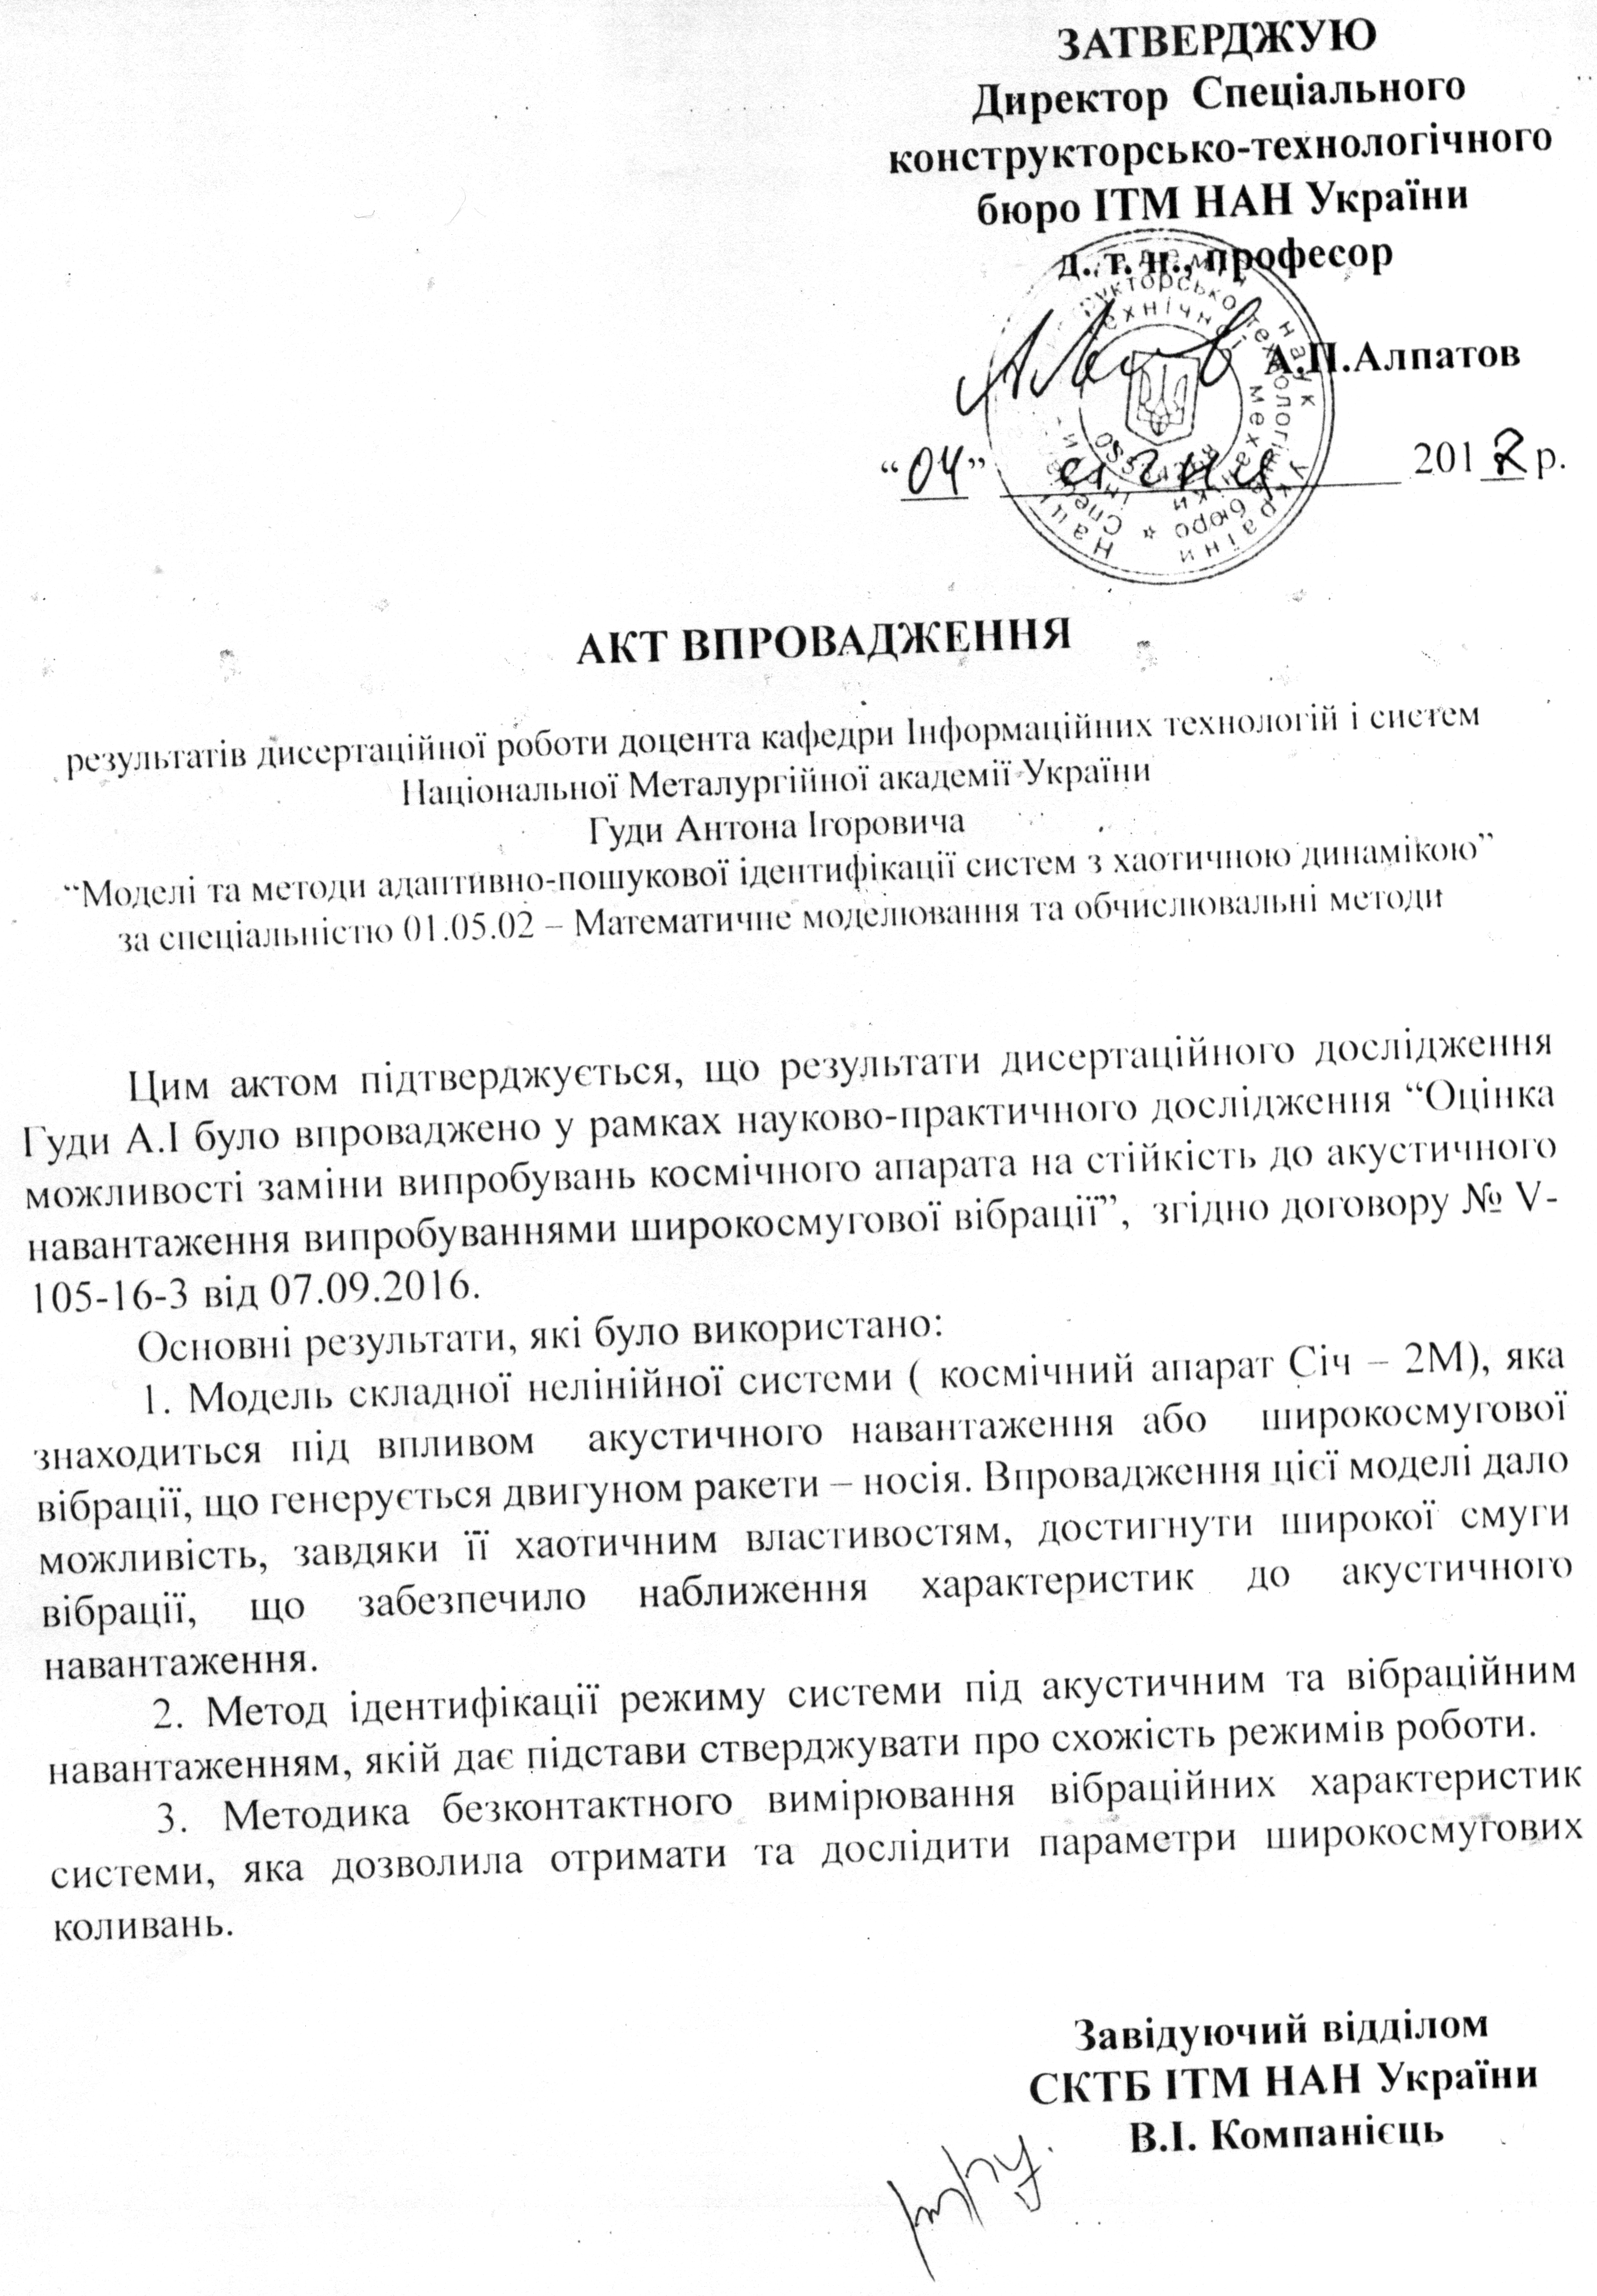
\includegraphics[width=0.98\textwidth]{sich2_akt.png}
%Акти впровадження дисертаційної роботи
\end{center}


\clearpage
\phantomsection
\vspace{-7ex}
\chapter*{Додаток Б}

\vspace{-5ex}
\begin{center}
%Акти впровадження дисертаційної роботи у навчаний процес
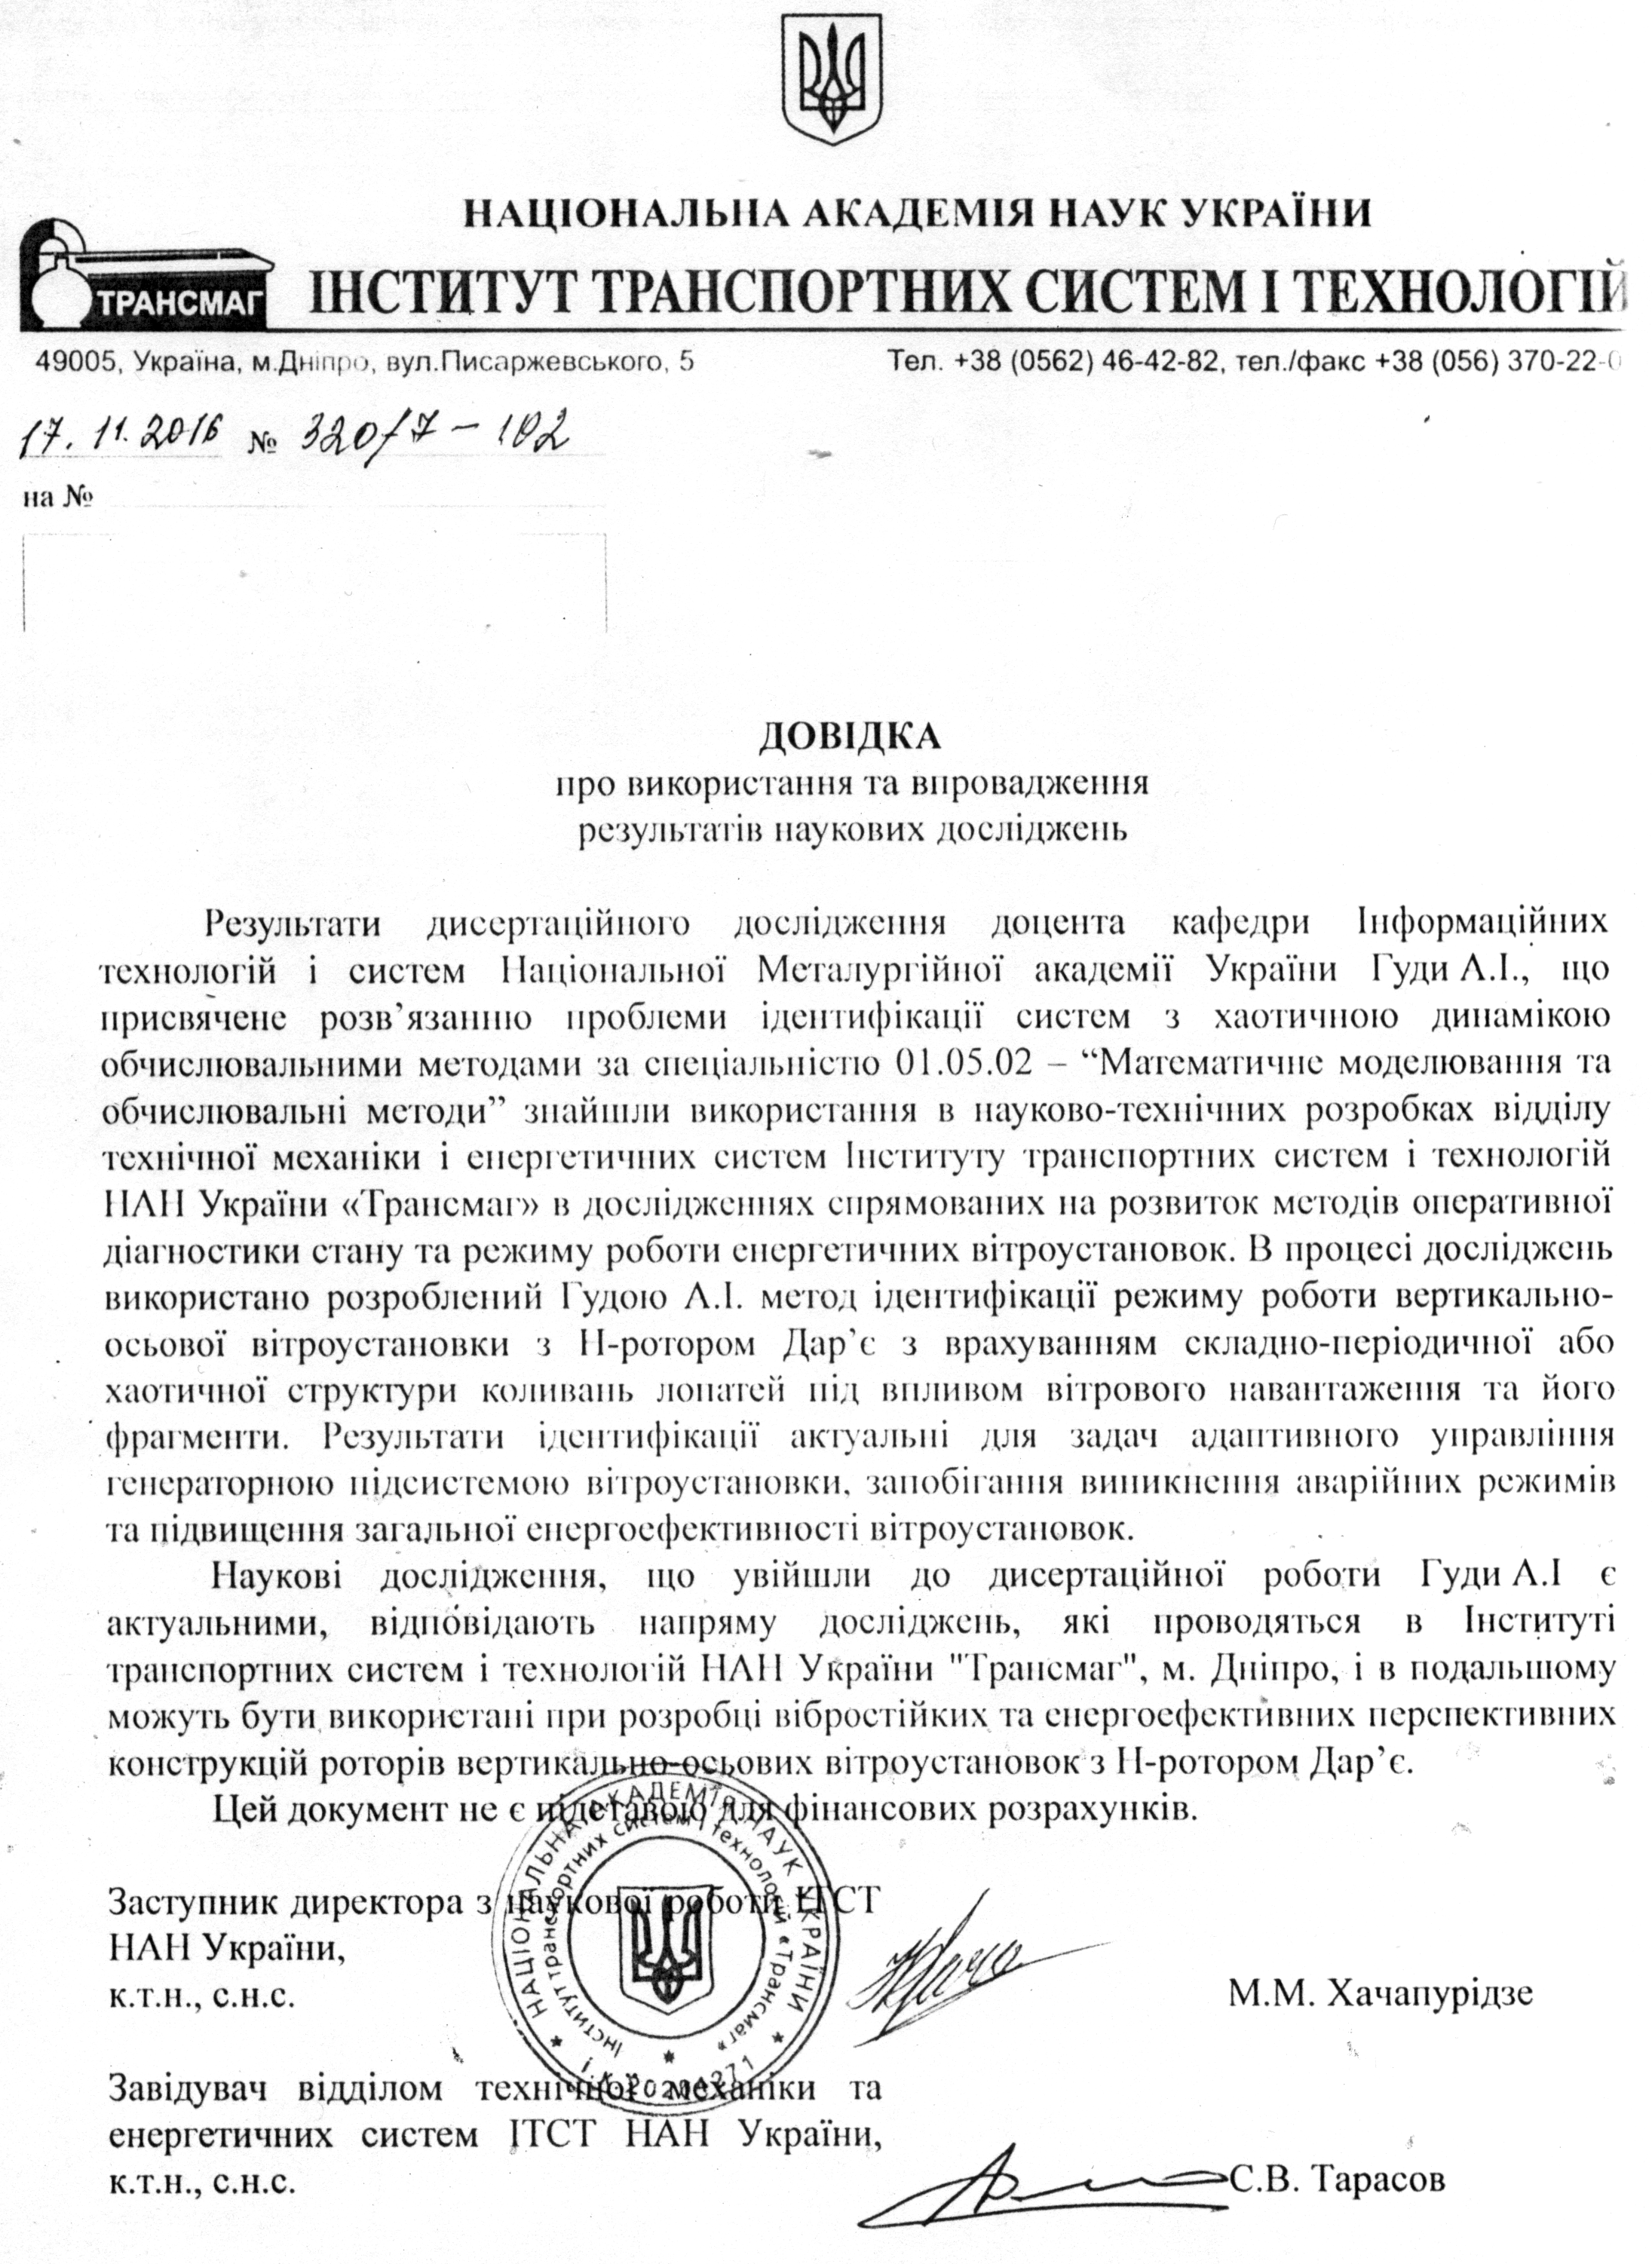
\includegraphics[width=0.98\textwidth]{transmag_dovidka.png}
\end{center}


\clearpage
\phantomsection
\chapter*{Додаток В}

\vspace{-7ex}
\begin{center}
  Список публікацій здобувача
\end{center}

\begin{enumerate}



\item
Гуда А. И., Михалёв А. И., Новикова Е. Ю. Синтез критерия идентификации нелинейных
динамических систем на физических принципах // Адаптивнi системи автоматичного
управлiння. Мiжвiдом. науково-техн. зб. (РИНЦ). --- Днепропетровск, 2008. --- 11(31). --- С. 136--142.

\item
Гуда А. И., Михалёв А. И. Адаптивно-поисковая идентификация хаотической динамической
системы Дуффинга // Адаптивнi системи автоматичного управлiння.
Мiжвiдом. науково-техн. зб. (РИНЦ). --- Днепропетровск, 2008. --- 12(32). --- С. 166--171.

\item
Гуда А. И., Михалёв А. И. Адаптивно-поисковая идентификация хаотической динамической
системы Рёсслера // Адаптивнi системи автоматичного управлiння. Мiжвiдом.
науково-техн. зб. (РИНЦ). --- Днепропетровск, 2009. --- 14(34). --- С. 125--129.

\item
Guda A. I., Mikhalyov A. I. Multi-model methods and parameters estimation approaches
on non-linear dynamic system identification // Системнi технологiї. Регiональний мiжвузiвський
збiрник наукових праць (Index Copernicus). --- Днепропетровск, 2015. --- 4(99). --- С. 3--9.

\item
Guda A. I., Mikhalyov A. I. Multi-model identification system properties near extremum:
simulations and analysis // Journal of Applied Computer Science – JACS-2015. --- 2015. --- 23(2). --- С. 21--28.

\item
Гуда А. И., Михалёв А. И. Выбор критерия при адаптивно-поисковой идентификации
динамической системы Ван-Дер-Поля // Адаптивнi системи автоматичного управлiння.
Мiжвiдом. науково-техн. зб. (РИНЦ). --- Днепропетровск, 2010. --- 16(36). --- С. 154--160.

\item
Гуда А. И., Михалёв А. И. Использование нечётких технологий при выборе начальных
условий в задачах идентификации систем с хаотической динамикой // Адаптивнi системи
автоматичного управлiння. Мiжвiдом. науково-техн. зб. (РИНЦ). --- Днепропетровск, 2014. --- 2(25). --- С. 98--103.

\item
Guda A. I., Mikhalyov A. I. Method of Lorenz systems parametric identification by the
searching models ensemble // Scientific and Technical Conference ``Computer Sciences and
Information Technologies'' (CSIT) (Scopus). --- 2015. --- С. 73--75. --- DOI: 10.1109/STC-CSIT.2015.7325435.

\item
Гуда А. И., Михалёв А. И. Информационные оценки сложности задачи параметрической
идентификации динамических систем // Адаптивнi системи автоматичного
управлiння. Мiжвiдом. науково-техн. зб. (РИНЦ). --- Днепропетровск, 2007. --- 10(30). --- С. 96--103.

\item
Гуда А. И., Михалёв А. И., Деревянко А. И. Критерии идентификации параметров хаотической
динамики управляемого объекта // Автомобiльний транспорт. – Вiсник Харкiвського
нацiонального автодорожнього унiверситету. --- 2009. --- No 25. --- С. 254--257.

\item
Гуда А. И., Михалёв А. И. Влияние возмущений входного сигнала на динамику и
идентификацию нелинейной системы Дуффинга // Адаптивнi системи автоматичного
управлiння. Мiжвiдом. науково-техн. зб. (РИНЦ). --- Днепропетровск, 2010. ---
15(35). --- С. 121--125.

\item
Гуда А. И., Михалёв А. И. Исследование альтернативного критерия при адаптивно-поисковой
идентификации динамической системы Ван-Дер-Поля // Адаптивнi системи автоматичного управлiння.
Мiжвiдом. науково-техн. зб. (РИНЦ). --- Днепропетровск, 2010. --- 17(37). --- С. 149--154.

\item
Гуда А. И., Михалёв А. И. Сравнительный анализ двух критериев адаптивно-поисковой
идентификации нелинейной динамической системи Ван-Дер-Поля // Системнi технологiї.
Регiональний мiжвузiвський збiрник наукових праць. --- Днепропетровск,
2011. --- 4(75). --- С. 15--20.

\item
Гуда А. И., Михалёв А. И. Синтез критерия при адаптивно-поисковой идентификации
динамической системы Чуа // Адаптивнi системи автоматичного управлiння. Мiжвiдом.
науково-техн. зб. (РИНЦ). --- Днепропетровск, 2011. --- 18(38). --- С. 140--146.

\item
Гуда А. И., Михалёв А. И., Дмитриева И. С. Особенности моделирования и идентификации
хаотической системы Ресслера с возмущениями // Системнi технологiї. Регiональний
мiжвузiвський збiрник наукових праць. --- Днепропетровск, 2010. --- 2(67). --- С. 114--118.

\item
Гуда А. И., Михалёв А. И. Моделирование и исследование хаотической динамики связанных
релаксационных генераторов // Адаптивнi системи автоматичного управлiння.
Мiжвiдом. науково-техн. зб. (РИНЦ). --- Днепропетровск, 2011. --- 19(39). --- С. 164--170.

\item
Гуда А. И., Михалёв А. И. Физические основы при синтезе критерия адаптивно-поисковой
идентификации динамической системы Лоренса // Системнi технологiї. Регiональний мiжвузiвський
збiрник наукових праць. --- Днепропетровск, 2012. --- 2(79). --- С. 13--19.

\item
Guda A. I., Mikhalyov A. I. Chaotic system with relay hysteresis in return force: simulation
and analysis // Системнi технологiї. Регiональний мiжвузiвський збiрник наукових
праць (Index Copernicus). --- Днепропетровск, 2013. --- 2(85). --- С. 30--35.

\item
Гуда А. И., Михалёв А. И. Моделирование хаотической динамики системы с зоной
нечувствительности и идентификация её параметров // Адаптивнi системи автоматичного
управлiння. Мiжвiдом. науково-техн. зб. (РИНЦ). --- Днепропетровск, 2012. ---
20(40). --- С. 180--186.

\item
Гуда А. И., Михалёв А. И. Генератор Колпитца: моделирование хаотической динамики
и параметрическая идентификация // Адаптивнi системи автоматичного управлiння.
Мiжвiдом. науково-техн. зб. (РИНЦ). --- Днепропетровск, 2012. --- 21(41). --- С. 146--153.

\item
Guda A. I., Mikhalyov A. I. Influence of input and measurement noise to Lorenz system
adaptive-searching identification // Системнi технологiї. Регiональний мiжвузiвський
збiрник наукових праць (Index Copernicus). --- Днепропетровск, 2014. --- 2(91). --- С. 154--158.

\item
Гуда А. И., Михалёв А. И. Настройка адаптивно-поисковой системы идентификации применительно
к хаотическим объектам // Адаптивнi системи автоматичного
управлiння. Мiжвiдом. науково-техн. зб. (РИНЦ). --- Днепропетровск, 2013. --- 1(22). ---
С. 134--139.

\item
Гуда А. И., Михалёв А. И. Расширение рабочего диапазона поисковой идентификации
нелинейных динамических систем // Адаптивнi системи автоматичного управлiння.
Мiжвiдом. науково-техн. зб. (РИНЦ). --- Днепропетровск, 2013. --- 2(23). --- С. 133--127.

\item
Гуда А. И., Михалёв А. И. Повышение качества фильтрации при поисковой идентификации
нелинейных динамических систем // Адаптивнi системи автоматичного
управлiння. Мiжвiдом. науково-техн. зб. (РИНЦ). --- Днепропетровск, 2014. --- 1(24). --- С. 160--165.

\item
Physical background in identification criterion synthesis / A. I. Guda, A. I. Mikhalyov,
A. I. Derevjanko, P. Kisa la // Elektronika konstrukcje, technologie, zastosowania (Index
Copernicus). --- 2013. --- No 8. --- С. 32--34.

\item
Гуда А. И., Михалёв А. И. Расширение рабочего диапазона при поисковой идентификации
хаотической системы Чуа // Вестник Херсонского национального технического
университета"(РИНЦ). --- 2014. --- 3(50). --- С. 265--258.

\item
Гуда А. И., Михалёв А. И. Использование метода идентификации с множеством
подвижных моделей применительно к динамической системе Лоренса // Адаптивнi системи
автоматичного управлiння. Мiжвiдом. науково-техн. зб. (РИНЦ). --- Днепропетровск, 2015.
--- 1(26). --- С. 191--197.

\item
Система поддержки принятия решений по повышению эффективности гидроаеродинамических
процессов во вспомогательных элементах энергетических агрегатов /
Е. А. Арсирий, С. Г. Антощук, В. А. Арсирий, А. И. Гуда // Управляющие системы и машины (РИНЦ).
--- 2015. --- No 6. --- С. 43--50.

\item
Гуда А. И., Михалёв А. И. Настройка параметров системы мультимодельной
адаптивно-поисковой системы идентификации // Вестник Херсонского национального
технического университета"(РИНЦ). --- 2015. --- 3(54). --- С. 138--243.

\item
Guda A. I., Mikhalyov A. I. Multi-model methods and parameters estimation approaches
on non-linear dynamic system identification // Системнi технологiї. Регiональний мiжвузiвський
збiрник наукових праць (Index Copernicus). --- Днепропетровск, 2016. --- 2(103). --- С. 57--62.

\item
Визначення гранулометричного складу матерiалу у повiтряному потоцi з використанням
дiаграм Пуанкаре / Р. О. Сухомлин, А. И. Михальов, Н. С. Прядко, К. В. Тернова, А. И. Гуда
// Системнi технологiї. Регiональний мiжвузiвський збiрник наукових
праць (Index Copernicus). --- Днепропетровск, 2016. --- 4(105). --- С. 18--24.

\item
Гуда А. И. A low-voltage coupled relaxation generator with chaotic behavior: simulation,
measurement and identification // Системнi технологiї. Регiональний мiжвузiвський
збiрник наукових праць (Index Copernicus). --- Днепропетровск, 2016. --- 4(105). --- С. 57--65.

\item
Guda A. I., Mikhalyov A. I. Three-model methods for extremum extimation in non-linear
dynamic system identification // Адаптивнi системи автоматичного управлiння.
Мiжвiдом. науково-техн. зб. (РИНЦ). --- Днепропетровск, 2016. --- 2(27). --- С. 160--165.

\item
Зимогляд А. Ю., Гуда А. И. Особливостi використання HX711 для отримання даних з
тензодатчика // Системнi технологiї. Регiональний мiжвузiвський збiрник наукових
праць (Index Copernicus). --- Днепропетровск, 2016. --- 3(104). --- С. 136--140.

\item
Левченко Д., Гуда А. И. Виявлення залежностi кута повороту сервоприводу вiд вхiдного
iмпульсу // Системнi технологiї. Регiональний мiжвузiвський збiрник наукових праць
(Index Copernicus). --- Днепропетровск, 2016. --- 3(104). --- С. 141--146.

\item
Гуда А. И., Михалёв А. И. Синтез критерия для идентификации хаотической системы ``Sprott A''
с использованием мультимодельного адаптивно-поискового метода //
Вестник Херсонского национального технического университета"(РИНЦ). --- Херсон,
2016. --- 3(58). --- С. 204--207.

\item
Guda A. I., Mikhalyov A. I. Multi-models identification methods comparison in the non-linear
dynamic system identification task // Радиоэлектроника, информатика, управление (Web of Science).
--- Запорiжжя, ЗНТУ, 2016. --- No 4. --- С. 112--119. --- DOI: 10 . 15588/1607-3274-2016-4-14.

\item
Гуда А. И., Михалёв А. И. Оценивание эффективности применения интегральных критериев в задачах
параметрической идентификации хаотических систем // Коллективная монография
``Системные технологии моделирования сложных систем'' под. ред.
Михалёва А.И. --- Днепр, 2016. --- С. 200--229.

\item
Гуда А. И., Михалёв А. И. Выбор критериев для оценки эффективности процессов идентификации
систем с хаотической динамикой // Матерiали Всеукраїнської науково-практичної конференцiї
``Iнформатика та системнi науки'' (IСН-2011).
--- Полтава, 17-19.03.2011. --- Полтава: РВВ ПУЕТ. --- 2011. --- С. 355.

\item
Гуда А. И., Михалёв А. И. Идентификация систем с хаотической динамикой
// Материалы международной конференции ``Интеллектуальные системы принятия решений и
проблемы вычислительного интеллекта'' (ISDMCI) (май 2011).
--- Херсон: ХНТУ : ХН-ТУ, 2011. --- С. 211--212.

\item
Гуда А. И., Михалёв А. И. Адаптивно-поисковая идентификация нелинейной динамической
системы Ван-дер-Поля // Информационные технологии в управлении сложными системами.
Сборник докладов научной конференции – Днепропетровск:
изд-во ``Свидлер А.Л.'' --- Днепропетровск, 07.2011. --- С. 39--40.

\item
Гуда А. И., Михалёв А. И. Адаптивно-поисковая идентификация нелинейной хаотической
системы Чуа // Материалы международной научно-технической конференции
``Автоматизация: проблемы, идеи, решения'' (сент. 2011). --- Севастополь : СевНТУ,
2011. --- С. 18--19.

\item
Гуда А. И., Михалёв А. И. Альтернативный критерий идентификации хаотической системы Рёсслера
// Материалы международной конференции ``Интеллектуальные системы принятия решений
и проблемы вычислительного интеллекта'' (ISDMCI). ---
Херсон: ХНТУ : ХНТУ, 2012. --- С. 247--249.

\item
Гуда А. И., Михалёв А. И. Синтез критерия идентификации нелинейной хаотической
системы Лоренса // Материалы международной научно-технической конференции
``Автоматизация: проблемы, идеи, решения'' (сент. 2012). --- Севастополь : СевНТУ,
2012. --- С. 11--13.

\item
Гуда А. И., Михалёв А. И. Хаотические колебательные системы с зоной нечувствительности
и релейным гистерезисом в восстанавливающей силе // Материалы международной конференции
``Интеллектуальные системы принятия решений и проблемы
вычислительного интеллекта'' (ISDMCI). --- Херсон: ХНТУ : ХНТУ, 2013. --- С. 434--435.

\item
Гуда А. И., Михалёв А. И. Идентификация бифуркационного параметра генератора
Колптица // Материалы международной научно-технической конференции
``Автоматизация: проблемы, идеи, решения'' (сент. 2013). --- Севастополь : СевНТУ, 2013. ---
С. 104--105.

\item
Гуда А. И., Михалёв А. И. Совместное влияние изменений параметров системы
адаптивно-поисковой идентификации хаотических систем объектов на процесс поиска
// Материалы международной конференции ``Интеллектуальные системы принятия
решений и проблемы вычислительного интеллекта'' (ISDMCI). --- Херсон: ХН-ТУ : ХНТУ, 2014. --- С. 63--64.

\item
Гуда А. И., Михалёв А. И. Применение многомодельного метода в задаче параметрической
идентификации хаотической системы Лоренса // Материалы международной
конференции ``Интеллектуальные системы принятия решений и проблемы вычислительного интеллекта''
(ISDMCI). --- Херсон: ХНТУ : ХНТУ, 2015. --- С. 53--54.

\item
Гуда А. И., Михалёв А. И. Применение различных функций качества идентификации
при использовании ансамбля поисковых агентов в задаче идентификации нелинейных
динамических систем // Материалы международной конференции
``Интеллектуальные системы принятия решений и проблемы вычислительного интеллекта''
(ISDMCI). --- Херсон: ХНТУ : ХНТУ, 2016. --- С. 53--54.

\item
Guda A. I., Mikhalyov A. I. Criteria synthesis problem for the chaotic systems identification //
Proceedings of the 2016 IEEE 1st International Conference on Data Stream Mining and
Processing, DSMP 2016, (Web of Science, Scopus, РИНЦ). --- Lviv, Ukraine, 08.2016. ---
С. 125--128.

\end{enumerate}

% vim: fdm=marker foldlevel=1 foldignore="%#" fdc=4 ft=tex



\end{document}

